\chapter{Design \& Specification}

As previously described, the project aims to create an extensible Lispish to JavaScript compiler. 
In order to ... we need to formalise our input language Lispish to clearly define the possible constructs that we allow in our program. 
As Lispish defines a subset of an existing language, it is therefore even more important to be clear on what it possible and what is not. 

\section{Designing the Lispish language}

Lispish is a dynamically typed, functional language that implements a call-by-value strategy just as its superset Clojure.

The formal description of Lispish behaviour will be described using transition systems.

\subsection{Grammar of Lispish}

$F \Coloneqq \ (let \ [x \ F] \ (F)) \\
| \	(if \ (F) \ F_1 \ F_2) \\
| \	(defn \ name \ [args*] \ (F)) \\
| \	(fn \ [arg] \ (F)) \\
| \	(cond \ (F_0) \ F_1 \ (F_2) \ F_3) \\
| \     T \\
| \     X
$

where
\\
$X \Coloneqq T $
\\
$T \Coloneqq \ () \ \vert \ N \ \vert \ B \ \vert \ s $
\\
$N \Coloneqq n \ \vert \ (op \ N \ N)  $
\\
$B \Coloneqq b\ \vert \ (bop \ t1 \ t2) \ $
\\
$op \Coloneqq \ + \ \vert \ - \ \vert \ * \ \vert \ /$
\\
$bop \Coloneqq \ > \vert < \vert =$
\\
$s \Coloneqq \ String $
\\
$n \Coloneqq \ Integer $
\\
$b \Coloneqq \ true \ \vert \ false $
\\
$() \Coloneqq \ List $

\subsection{Evaluation relations (Big-Step Semantics)}
Operators:
\[
\inference[bop]{E_1, s \ $$\Downarrow$$ \ b_1, s' \ E_2, s' \ $$\Downarrow$$ \ b_2, s''}
{(bop \ E_1 \ E_2) \ $$\Downarrow$$ \ b, s'', if (= b \ (bop \ b_1 \ b_2))}
\]
\[
\inference[op]{E_1, s \ $$\Downarrow$$ \ n_1, s' \ E_2, s' \ $$\Downarrow$$ \ n_2, s''}
{(op \ E_1 \ E_2) \ $$\Downarrow$$ \ b, s'', if (= b \ (op \ n_1 \ n_2))}
\]


Atomic:

\[
\inference[String]{}
{s \ $$\Downarrow$$ \ s}
\]
\[
\inference[Integer]{}
{n \ $$\Downarrow$$ \ n}
\]
\[
\inference[List]{n \ $$\Downarrow$$ \ v}
{(n) \ $$\Downarrow$$ \ v}
\]
Forms (F):
\[
\inference[let]{t_0 \ $$\Downarrow$$ \ v}
{(\text{let } \ {[x \ (t_0)]} \ (t_1)) \ $$\Downarrow$$ \ t_1 {[}x \ $$\mapsto$$ \ v{]} }
\]
\[
\inference[if true]{{t_0} \ $$\Downarrow$$ \ \textsc{True} & t_1 \ $$\Downarrow$$ \ v}
{(if \ (t_0) \ t_1 \ t_2) \ $$\Downarrow$$ \ v) }
\]
\[
\inference[if false]{t_0 \ $$\Downarrow$$ \ \textsc{False} & t2 \ $$\Downarrow$$ \ v}
{(if \ (t_0) \ t_1 \ t_2) \ $$\Downarrow$$ \ v) }
\]
\[
\inference[cond]{t_0 \ $$\Downarrow$$ \ \textsc{False} & t_1 \ $$\Downarrow$$ \ \textsc{True} & t_3 \ $$\Downarrow$$ \ v}
{(cond \ (t_0) \ t_2 \ (t_1) \ t_3) \ $$\Downarrow$$ \ v) }
\]
\[
\inference[defn]{ {t_0 \ [x]} \ $$\Downarrow$$ \ v}
{(defn \ s \ {[x]} \ (t_0)) \ $$\Downarrow$$ \ s \ $$\mapsto$$ \ v }
\]
\[
\inference[fn]{ {t_0 \ [x]} \ $$\Downarrow$$ \ v}
{(fn \ {[x]}  \ (t_0) \ $$\Downarrow$$ \ v }
\]

\section{Development methodology}
In order to streamline the process of development of the compiler, I have decided to use the Test Driven Development (TDD) methodology that emphasizes on building small units of functionalities that can be invidually tested by designeted unit tests. 

Clojure allows developers to create programs using the REPL (Read Evaluation Print Loop), which is characteristic feature in new dynamic programming languages. It allows you to write your functions, evaluate them and get an instant result from an interpreter that interacts with your code. This in essence reduces the amount of unit tests that have to be implemented for trivial functions in a TDD project. 
REPL is a great resource for rapid development and prototyping of functions, but also ensuring that they yield the right result before the project as a whole is compiled.

\subsection{Unit tests}
Even though Clojure provides REPL, it is still important to develop a regression testing suite that ensures whenever the compiler is modified, it can still compile and yield the same result for old programs.
To do this, I will use clojure.test API that provides a set of macros for evaluating forms and ensuring they yield the expected result. 

\section{Compiling Lispish to JavaScript (Compiler design??)}

\subsection{Compilation pipeline (use case/state machines?)}

\begin{figure}[hb]
	\centering
	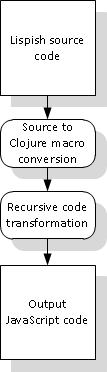
\includegraphics{Graphics/test.jpg}
	\caption[Abstract \textit{Lispish to JavaScript} compilation.]
   {Abstract figure of \textit{Lispish to JavaScript} compilation.}
\end{figure}

The compiler in its simplest form will perform a one to one translation in-line translation from Lispish to JavaScript. 
The input source will be treated by a macro function that will prevent the code from being evaluated and it will pass it along down the pipeline to its respective emitters as ilustrated on figure ~\ref{fig:abstract_compilation}. Code will be treated as data and I will use the prefix notation to my advantage, treating each expression as its respective node in a parse tree. 

\subsection{Alternative approach}
